\chapter{Resultados Preliminares}
\label{cap:resultados}

Este capítulo reporta os resultados já obtidos, suficientes para sustentar a
viabilidade da proposta e, igualmente, para delimitar os regimes em que o
indicador não se sustenta. Todos os números foram recalculados a partir dos
registros por época das execuções, e não reproduzidos de análises anteriores.

\section{Protocolo Experimental}
\label{sec:R-protocolo}

Os experimentos utilizam o repositório MedNIST, com a arquitetura ResNet-18
\cite{he2016} e, para o teste de generalização entre arquiteturas, a
DenseNet-121. A partição em treino, validação e teste é congelada e reutilizada
entre execuções, de modo que a comparação entre elas não seja contaminada por
variação de amostragem.

A memorização é induzida pela corrupção de uma fração dos rótulos do conjunto
de treino, seguindo o protocolo de \citeonline{zhang2017}. Cada execução com
corrupção possui uma execução de controle pareada, idêntica em tudo exceto pela
ausência de corrupção. A semente que governa a corrupção é independente daquela
que governa a partição e a inicialização --- distinção necessária, pois, se
ambas fossem a mesma, repetir o experimento com semente diferente reproduziria
exatamente os mesmos rótulos errados e mediria sensibilidade à inicialização,
não replicação.

O conjunto principal de resultados compreende oito execuções com corrupção de
30\% dos rótulos e oito execuções de controle, todas com ResNet-18.

\section{Discriminação entre Memorização e Aprendizado}
\label{sec:R-discriminacao}

A Tabela~\ref{tab:discriminacao} apresenta a amplitude de variação de cada
indicador ao longo do treinamento, comparada entre os dois grupos. A razão entre
as médias é o que importa: um indicador que varia muito nas duas condições não
informa nada sobre a memorização.

\begin{table}[H]
    \centering
    \caption{Amplitude de variação dos indicadores em execuções com corrupção
    de rótulos e em controles pareados ($n = 8$ por grupo). Valores como
    média $\pm$ desvio-padrão amostral; $p$ obtido por teste de
    Mann-Whitney bilateral.}
    \label{tab:discriminacao}
    \begin{tabular}{lcccc}
        \toprule
        Indicador & Com corrupção & Controle & Razão & $p$ \\
        \midrule
        LMC       & \num{1,219} $\pm$ \num{0,055} & \num{1,153} $\pm$ \num{0,130} & \num{1,06} & \num{0,33} \\
        SampEn 1D & \num{0,205} $\pm$ \num{0,018} & \num{0,056} $\pm$ \num{0,009} & \num{3,64} & \num{0,00016} \\
        SampEn2D  & \num{0,340} $\pm$ \num{0,061} & \num{0,060} $\pm$ \num{0,008} & \num{5,71} & \num{0,00016} \\
        \bottomrule
    \end{tabular}
    \fonte{Elaborado pelo autor.}
\end{table}

O resultado é assimétrico e merece ser lido com atenção. A complexidade LMC
\textbf{não discrimina} as duas condições: a razão de \num{1,06} é
compatível com ausência de efeito e o teste não rejeita a hipótese nula
($p = \num{0,33}$). Como discutido na Seção~\ref{sec:T-complexidade}, a LMC é
invariante a permutações e lê apenas o histograma dos valores dos pesos; a
interpretação mais econômica desse achado é que a memorização reorganiza os
pesos sem alterar substancialmente a distribuição de seus valores.

As duas variantes de entropia amostral discriminam, e a bidimensional
discrimina melhor. O valor $p = \num{0,00016}$ é o menor alcançável pelo teste
com $n = 8$ por grupo e corresponde à separação completa entre os grupos.

\section{Antecedência em Relação à Degradação da Validação}
\label{sec:R-antecedencia}

A antecedência é a diferença, em épocas, entre a inflexão do indicador e a
âncora definida sobre a acurácia de validação. A Tabela~\ref{tab:antecedencia}
reporta os valores obtidos.

\begin{table}[H]
    \centering
    \caption{Antecedência dos indicadores em relação à queda sustentada da
    acurácia de validação, em épocas, nas oito execuções com corrupção.}
    \label{tab:antecedencia}
    \begin{tabular}{lccc}
        \toprule
        Indicador & Média $\pm$ desvio & IC \SI{95}{\percent} & Discrimina? \\
        \midrule
        SampEn2D  & \num{7,50} $\pm$ \num{0,93} & [\num{6,73};\ \num{8,27}] & Sim \\
        SampEn 1D & \num{3,62} $\pm$ \num{1,06} & [\num{2,74};\ \num{4,51}] & Sim \\
        LMC       & \num{3,00} $\pm$ \num{1,85} & [\num{1,45};\ \num{4,55}] & Não \\
        \bottomrule
    \end{tabular}
    \fonte{Elaborado pelo autor.}
\end{table}

Registre-se que a antecedência da LMC não deve ser interpretada como resultado
positivo: como a Tabela~\ref{tab:discriminacao} mostra que o indicador não
distingue as duas condições, a época de sua inflexão não constitui aviso de
coisa alguma. A antecedência só é informativa para indicadores que discriminam.

A separação temporal da SampEn2D é limpa. Nas oito execuções com corrupção, o
indicador inflete nas épocas $\{7,7,7,7,7,7,8,9\}$; nos controles em que chega a
inflectir, isso ocorre entre as épocas \num{13} e \num{31}, e em duas das oito
execuções de controle não há inflexão alguma dentro do horizonte de treinamento.
Não há sobreposição entre as duas distribuições.

\begin{figure}[H]
    \centering
    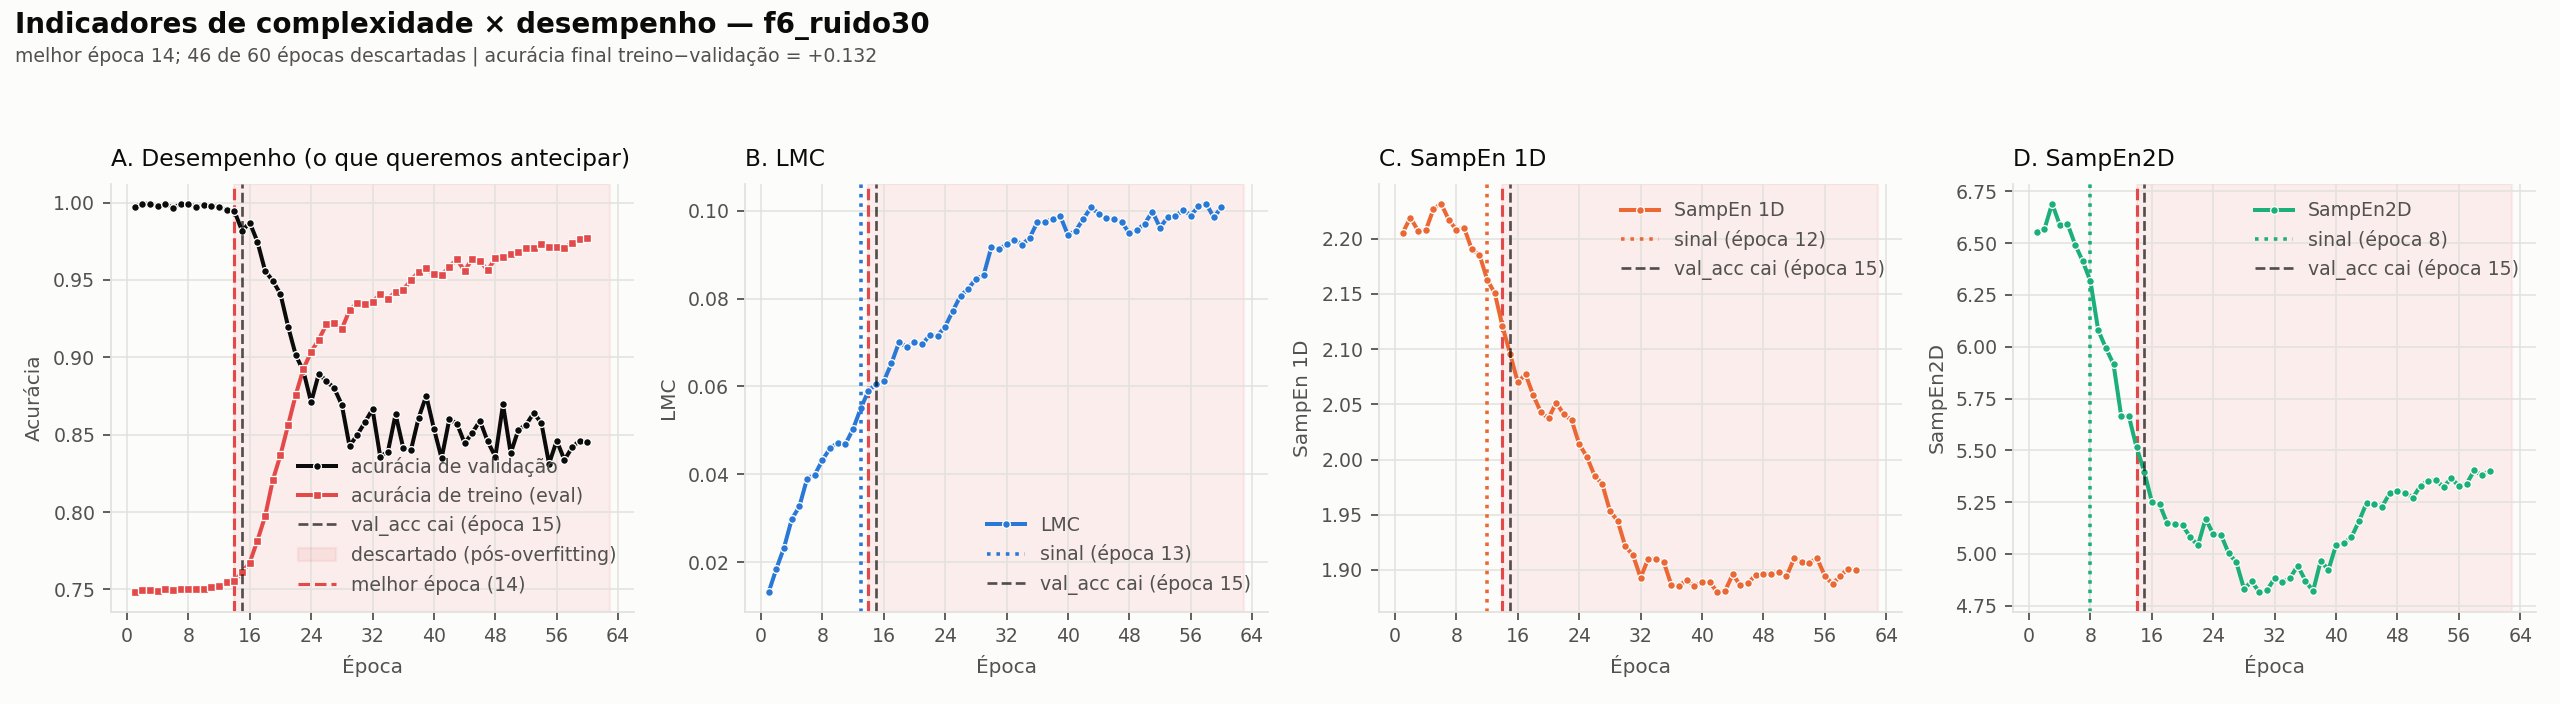
\includegraphics[width=0.95\textwidth]{figuras/indicadores_f6_ruido30.png}
    \caption{Trajetória dos três indicadores e da validação em execução com
    corrupção de \SI{30}{\percent} dos rótulos. A região sombreada corresponde
    às épocas posteriores ao início do \emph{overfitting}, excluídas das
    conclusões.}
    \label{fig:indicadores}
    \fonte{Elaborado pelo autor.}
\end{figure}

\section{Efeito do Nível de Corrupção}
\label{sec:R-niveis}

Variou-se a fração de rótulos corrompidos em \SI{15}{\percent},
\SI{30}{\percent} e \SI{50}{\percent}, com três sementes por nível. O resultado
é instrutivo e não era o esperado.

A época em que o monitor emite o alerta é praticamente invariante ao nível de
corrupção --- médias de \num{10,0}, \num{9,3} e \num{10,0} épocas para os três
níveis, sem diferença estatisticamente detectável
($F = \num{1,00}$; $p = \num{0,42}$). O que se move é a âncora, isto é, o momento
em que a degradação se torna visível na validação, que chega progressivamente
mais cedo com mais corrupção ($F = \num{30,2}$; $p = \num{0,0007}$).

A consequência prática é que a antecedência encolhe à medida que a corrupção
aumenta: aproximadamente \num{7,7} épocas a \SI{15}{\percent}, \num{5,3} a
\SI{30}{\percent} e \num{3,0} a \SI{50}{\percent}. A leitura que se propõe é
que o indicador marca o \emph{início} da memorização, cujo momento depende pouco
da quantidade de rótulos errados, enquanto a validação mede o \emph{sintoma},
que se manifesta tanto mais cedo quanto maior a corrupção. Trata-se de
interpretação plausível, ainda não demonstrada, e que o trabalho pretende
investigar.

\section{Generalização entre Arquiteturas: um Limite Identificado}
\label{sec:R-arquitetura}

O experimento foi repetido com DenseNet-121, em três execuções com corrupção e
três controles. Os resultados são parcialmente favoráveis e devem ser
reportados com precisão.

A antecedência é preservada e de fato ampliada: a SampEn2D inflete \num{20},
\num{21} e \num{17} épocas antes da âncora nas três execuções. Contudo, o poder
de discriminação por amplitude \textbf{cai substancialmente}: a razão entre
execuções com corrupção e controles é de \num{2,8} vezes, contra \num{5,71} na
ResNet-18, e as demais medidas deixam de discriminar (\num{1,3} para a
SampEn 1D e \num{1,2} para a LMC). Com três execuções por grupo, não há poder
estatístico para afirmar significância.

A conclusão honesta é que o achado central foi verificado em uma segunda
arquitetura quanto à antecedência, mas não quanto à magnitude do contraste. Se
isso decorre do tamanho da camada densa, da dinâmica de otimização própria da
DenseNet ou simplesmente do número reduzido de execuções, é questão em aberto e
consta entre os objetivos específicos deste projeto.

\section{Escolha da Âncora}
\label{sec:R-ancora}

Um resultado metodológico merece registro. A primeira versão do monitor ancorava
o diagnóstico na perda de validação. Nessa configuração, o monitor acusava
\emph{overfitting} em dez de dez execuções, incluindo todos os controles,
sinalizando o estado em cerca de metade das épocas mesmo quando não havia
corrupção alguma. A causa é que o MedNIST satura muito cedo, e a perda de
validação começa a subir logo após a primeira época mesmo em treinamentos
saudáveis.

Reancorando o diagnóstico na acurácia de validação, o comportamento tornou-se
o esperado: oito de oito execuções com corrupção sinalizadas, nenhum falso
positivo entre os oito controles. O episódio ilustra que a definição
operacional de \emph{overfitting} não é detalhe de implementação, mas condição
de validade do resultado.

\section{Limitações dos Resultados Atuais}
\label{sec:R-limitacoes}

\begin{enumerate}
    \item Os experimentos restringem-se a um único repositório de imagens, que
          é reconhecidamente fácil e satura rapidamente. A extensão a
          repositórios mais difíceis é necessária.
    \item A memorização é induzida artificialmente. Resta demonstrar que o
          indicador se comporta do mesmo modo diante de \emph{overfitting}
          espontâneo, por escassez de dados e não por corrupção de rótulos.
    \item O contraste em DenseNet-121 é fraco e baseado em três execuções por
          grupo.
    \item Os limiares do monitor foram calibrados em um subconjunto das
          execuções e verificados nas demais; ainda assim, a possibilidade de
          ajuste excessivo do critério aos próprios dados exige validação em
          condições inteiramente novas.
\end{enumerate}
